\color{black}



\begin{textblock}{16}(0,2)

\begin{figure}
    \centering
    \begin{tikzpicture}

\node[inner sep=0pt] (motherboard) at (3,0)
    {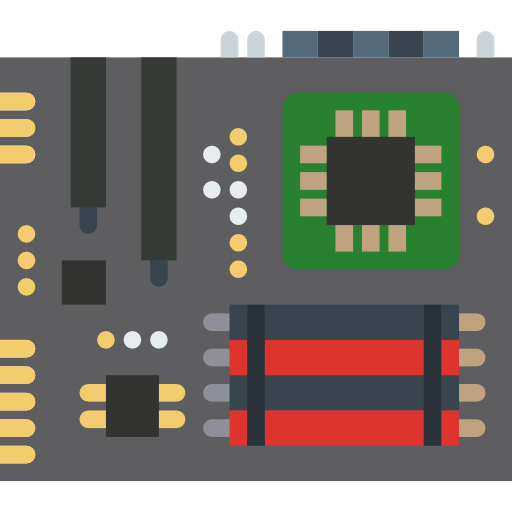
\includegraphics[width=.12\textwidth]{Simulation_sayem/pictures/motherboard.png}};  
\node[inner sep=0pt] (videocard) at (3,3)
    {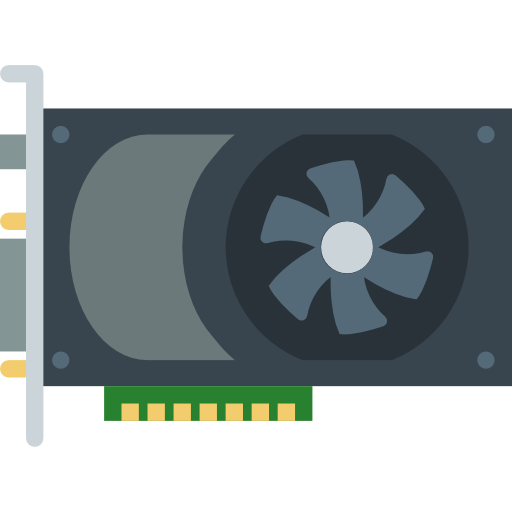
\includegraphics[width=.12\textwidth]{Simulation_sayem/pictures/video-card.png}};
    
\node[inner sep=0pt] (memory) at (0,0)
    {
\includegraphics[width=.12\textwidth]{Simulation_sayem/pictures/memory.png}};
    
\node[inner sep=0pt] (casing) at (6,0)
    {
\includegraphics[width=.12\textwidth]{Simulation_sayem/pictures/casing.jpg}};
\node[inner sep=0pt] (PSU) at (6,3)
    {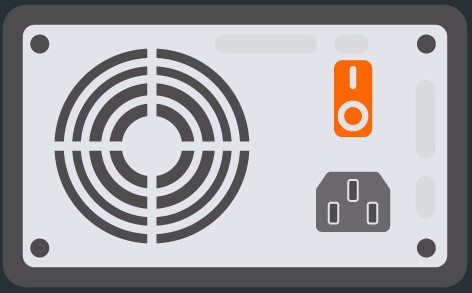
\includegraphics[width=.12\textwidth]{Simulation_sayem/pictures/powerSupply.jpg}};
\node[inner sep=0pt] (CPU) at (0,3) {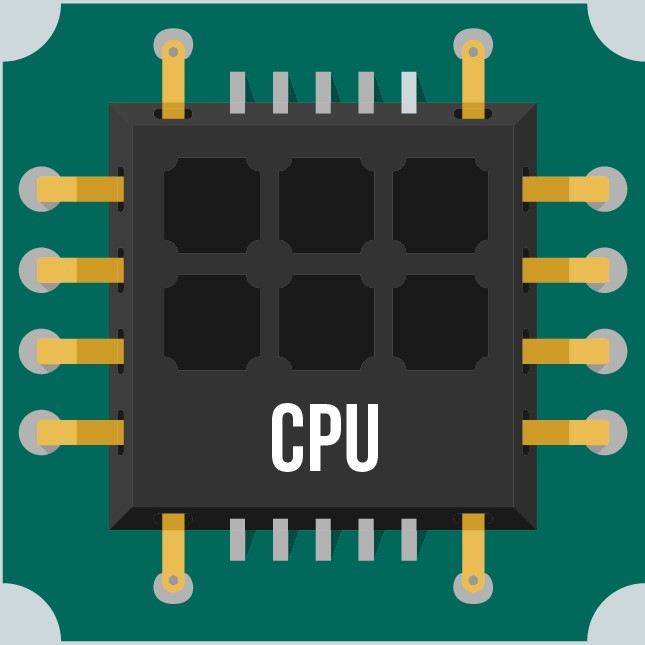
\includegraphics[width=.08\textwidth]{Simulation_sayem/pictures/processor.jpg}};


\node<3>[inner sep=0pt] (casingcross) at (6,0)
    {
\includegraphics[width=.12\textwidth]{Simulation_sayem/pictures/cross.png}};
\node<6>[inner sep=0pt] (memorycross) at (0,0)
    {
\includegraphics[width=.12\textwidth]{Simulation_sayem/pictures/cross.png}};


\draw<4-> [inactive edge] (PSU) --(casing);
\draw<4-> [inactive edge] (motherboard) --(casing);
\draw<10-> [inactive edge] (videocard) --(PSU);
\draw<8-> [inactive edge] (motherboard) --(videocard);
\draw<8-> [inactive edge] (CPU) --(videocard);
\draw<9-> [inactive edge] (motherboard) --(CPU);
\draw<7-> [inactive edge] (motherboard) --(memory);

\end{tikzpicture}
\end{figure}
\end{textblock}

\begin{textblock}{14}(5,12)
\begin{figure}
    \centering
    \begin{itemize}
        \only<2>{
        \vfill \item<2> Lets buy casing first }
        \only<3>{
        \vfill \item<3> But we can't!! }
        \only<4>{
        \vfill \item<4> We need motherboard and PSU model }
        \only<5>{
        \vfill \item<5> Lets try to buy RAM }
        \only<6>{
        \vfill \item<6> Again!! We can't }
        \only<7>{
        \vfill \item<7> We need motherboard model }
    \end{itemize}
\end{figure}
    
\end{textblock}